\section{Objective}
\label{sec:4-1}

Data Understanding and Data Preparation (Chapter~\ref{ch:data-preparation}) form one narrative: understand the data, extract findings about the reviews, and turn them into decisions for building the modelling dataset -- its metric, input, split and loss. The business question behind this chapter is which properties of the data must shape the models and their evaluation.

This chapter covers the first half of the narrative: an overview of the data (Section~\ref{sec:4-2}), class distribution (Section~\ref{sec:4-3}), text length (Section~\ref{sec:4-4}), change over time (Section~\ref{sec:4-5}), users, products and helpfulness (Section~\ref{sec:4-6}), noise in the text (Section~\ref{sec:4-7}) and the vocabulary of each class (Section~\ref{sec:4-8}). It ends with the design decisions (Section~\ref{sec:4-9}) that Chapter~\ref{ch:data-preparation} implements. Unless stated otherwise, all figures are measured on the cleaned table of 393{,}577 reviews produced in Section~\ref{sec:5-2}.

\section{Dataset Overview}
\label{sec:4-2}

\begin{center}
\begin{tabular}{@{}p{6cm}p{7.5cm}@{}}
    \toprule
    Metric & Value \\
    \midrule
    Rows in the raw file & 568{,}454 \\
    Rows after cleaning & 393{,}577 (69.2\% of raw) \\
    Distinct users (cleaned) & 256{,}044 \\
    Distinct products (cleaned) & 67{,}554 \\
    Date range & October 1999 -- October 2012 \\
    \bottomrule
\end{tabular}
\end{center}

\section{Class Distribution}
\label{sec:4-3}

The data lean heavily to the positive side. Positive reviews are roughly 78\% of the data, negative 14.5\% and neutral 7.6\%, so positive outnumbers neutral by about 10.3 to 1. A trivial classifier that always answers \emph{positive} reaches about 78\% accuracy yet only 0.29 Macro-F1, because the F1 of the other two classes is zero.

This is why Macro-F1 is the main metric (Section~\ref{sec:2-4}), and why the split is stratified and the loss is weighted (Chapter~\ref{ch:data-preparation}).

\section{Text Length}
\label{sec:4-4}

Review length is strongly right-skewed: the median body has 57 words but the longest has 3{,}432.

\begin{center}
\small
\begin{tabular}{@{}lrrrrrrrr@{}}
    \toprule
     & Mean & Std & Min & Median & P90 & P95 & P99 & Max \\
    \midrule
    \texttt{Text} (words) & 79.8 & 77.2 & 3 & 57 & 159 & 215 & 377 & 3{,}432 \\
    \texttt{Summary} (words) & 4.1 & 2.6 & 0 & 3 & 8 & 9 & 12 & 42 \\
    \bottomrule
\end{tabular}
\end{center}

Titles are short (median 3 words) but dense, for example ``Great taffy'' or ``Not as Advertised'', so the title is placed in front of the body to form the model input. Reviews with 2 or 3 stars tend to be longer than those with 5 stars, because the author explains both strengths and weaknesses.

A maximum of 200 words covers about 93\% of reviews without truncation, so it is used as the sequence limit for the BiLSTM. For the Transformer the limit is 256 subword tokens; the share of reviews it truncates (about 6.2\%) is measured in Section~\ref{sec:6-5}. When a review is cut, the end is lost and the beginning, which holds the title, is kept. Because lengths differ so much, batches use dynamic padding and length bucketing, so short reviews are not padded to the length of a 3{,}000-word outlier.

\section{Change over Time}
\label{sec:4-5}

\begin{center}
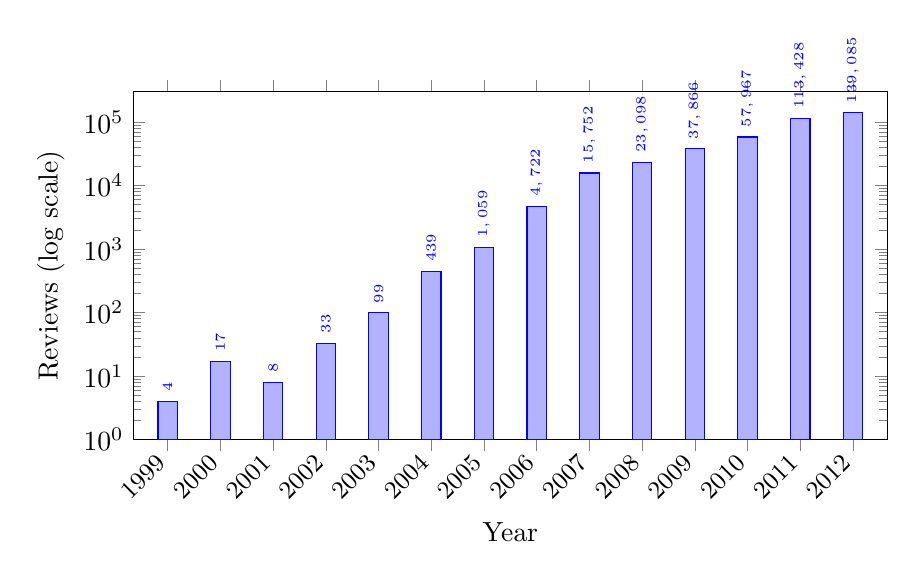
\begin{tikzpicture}
\begin{axis}[
  ybar, ymode=log, ymin=1, ymax=300000,
  width=0.92\textwidth, height=6cm,
  bar width=7pt,
  xlabel={Year}, ylabel={Reviews (log scale)},
  symbolic x coords={1999,2000,2001,2002,2003,2004,2005,2006,2007,2008,2009,2010,2011,2012},
  xtick=data, x tick label style={rotate=45,anchor=east,font=\small},
  point meta=explicit,
  nodes near coords={\pgfmathprintnumber[fixed,precision=0,1000 sep={,}]{\pgfplotspointmeta}},
  nodes near coords style={font=\tiny,rotate=90,anchor=west},
  enlarge x limits=0.05
]
\addplot coordinates {(1999,4) [4] (2000,17) [17] (2001,8) [8] (2002,33) [33] (2003,99) [99] (2004,439) [439] (2005,1059) [1059] (2006,4722) [4722] (2007,15752) [15752] (2008,23098) [23098] (2009,37866) [37866] (2010,57967) [57967] (2011,113428) [113428] (2012,139085) [139085]};
\end{axis}
\end{tikzpicture}
\end{center}

The number of cleaned reviews grows roughly exponentially from 2006, and 2011--2012 together hold 252{,}513 reviews (64.2\%); 2012 ends in October. The mean star rating drifts down from 4.386 in 2007 to 4.112 in 2012, and the negative share rises from 10.0\% to 16.1\%. The label distribution is therefore not stable in time.

The split in Section~\ref{sec:5-5} is random, so training and test reviews come from the same period. This does not measure how a model would fare on future reviews, and is listed as a limitation.

\section{Users, Products and Helpfulness}
\label{sec:4-6}

There are 256{,}044 distinct users and 67{,}554 distinct products. Of the users, 80.3\% wrote a single review, and 78.7\% of the products have five reviews or fewer. Both distributions have a long tail, so a model cannot rely on a user's rating habits and has to learn from the text.

Among reviews with at least five votes, negative reviews attract more votes but a lower helpful ratio, because readers often disagree with a complaint. Since this information is not available when a review is posted, it is not used as a feature (Section~\ref{sec:3-5}).

\section{Noise in the Text}
\label{sec:4-7}

\begin{center}
\begin{tabular}{@{}p{8cm}p{3cm}@{}}
    \toprule
    Noise in \texttt{Text} & Share of reviews \\
    \midrule
    HTML tags (mostly \texttt{<br />}) & 26.14\% \\
    URLs (\texttt{http}, \texttt{www}) & 2.08\% \\
    Encoded HTML characters (\texttt{\&amp;}, \texttt{\&quot;}) & 0.33\% \\
    \bottomrule
\end{tabular}
\end{center}

The text is therefore cleaned lightly (Section~\ref{sec:5-3}). Stop words and punctuation are \emph{kept}, because negations such as \emph{not}, \emph{no} and \emph{never} appear in standard stop-word lists but decide the sentiment, and because the neural models can learn the role of each word from context.

\section{Vocabulary of Each Class}
\label{sec:4-8}

Counting words and word pairs on a class-balanced sample of 20{,}000 reviews per class (stop words removed except negations) shows that single words such as \emph{like}, \emph{taste}, \emph{good} and \emph{coffee} occur in all three classes; \emph{good} is frequent even in negative reviews (``not good'', ``good but\ldots''). Word pairs separate the classes better: \emph{highly recommend}, \emph{great product} and \emph{love this} in positive reviews; \emph{waste money}, \emph{would not} and \emph{not buy} in negative ones. The neutral class has no vocabulary of its own and mixes that of the other two, so it is expected to be the hardest class.

\section{Design Decisions for Data Preparation}
\label{sec:4-9}

\begin{center}
\begin{tabular}{@{}p{6.2cm}p{7.9cm}@{}}
    \toprule
    Finding & Decision \\
    \midrule
    About 31\% of raw rows are repeated reviews & Remove them before splitting \\
    Labels skewed 77.9 / 14.5 / 7.6\% & Stratified split; class weights in the loss; Macro-F1 as main metric \\
    Right-skewed length; 200 words $\approx$ 93\% coverage & Limit of 200 words (BiLSTM) and 256 tokens (Transformer); dynamic padding and bucketing \\
    Titles are short but informative & Input is title followed by body \\
    26\% of bodies contain HTML & Light cleaning; keep punctuation and negations \\
    Context and negation matter & Use a sequence model (BiLSTM with attention) and a Transformer \\
    Label distribution drifts over time & Report as a limitation; the split is random \\
    \bottomrule
\end{tabular}
\end{center}
